% Author : Ali Snedden
% Date   : 9/10/19
% Compile:
%   pdflatex -shell-escape nerd_hour_09_13_2019.tex


\documentclass{beamer}
%\usetheme{Ilmenau}
\usetheme{Copenhagen}
%\usecolortheme{seahorse}
% See http://www.hartwork.org/beamer-theme-matrix/ for more themes and colors

% for themes, etc.
%\mode<presentation>{ \usetheme{boxes} }
%\mode<presentation>{ \usetheme{Warsaw} }
%\renewcommand*{\bibfont}{\scriptsize}

\usepackage{times}  % fonts are up to you
\usepackage{graphics}
\usepackage{amsmath}
\usepackage[makeroom]{cancel}
\usepackage{media9}
\usepackage{hyperref}
\usepackage{movie15}
\usepackage{epstopdf}

\usepackage{tikz}
\usetikzlibrary{fit}

\usepackage[absolute,overlay]{textpos}
\usepackage{psfrag}

%http://tex.stackexchange.com/questions/302584/problems-related-to-beamer-footcite
\makeatletter
\def\@iiiminipage#1#2[#3]#4{%
    \leavevmode
    \@pboxswfalse
    \setlength\@tempdima{#4}%
    \def\@mpargs{{#1}{#2}[#3]{#4}}%
    \setbox\@tempboxa\vbox\bgroup
    \color@begingroup
    \hsize\@tempdima
    \textwidth\hsize \columnwidth\hsize
    \@parboxrestore
    \let\@footnotetext\@mpfootnotetext
    \let\@listdepth\@mplistdepth \@mplistdepth\z@
    \@minipagerestore
    \@setminipage}
\makeatother

%http://tex.stackexchange.com/questions/138744/how-do-i-remove-citation-number-from-footcite
%\newcommand\footcitenonum[1]{%
%  \begingroup
%  \renewcommand\thefootnote{}\footnote{#1}%
%  \addtocounter{footnote}{-1}%
%  \endgroup
%}
%
%\makeatletter
%\renewrobustcmd{\blx@mkbibfootnote}[2]{%
%  \iftoggle{blx@footnote}
%    {\blx@warning{Nested notes}%
%     \addspace\mkbibparens{#2}}
%    {\unspace
%     \ifnum\blx@notetype=\tw@
%       \expandafter\@firstoftwo
%     \else
%       \expandafter\@secondoftwo
%     \fi
%       {\csuse{blx@theendnote#1}{\protecting{\blxmkbibnote{end}{#2}}}}
%       {\csuse{footnotenonum#1}{\protecting{\blxmkbibnote{foot}{#2}}}}}}
%\makeatother

%Bibliography stuff
%\usepackage[style=verbose,autocite=footnote,maxnames=10,babel=hyphen,hyperref=true,abbreviate=false,backend=biber,mcite]{biblatex}

\usepackage[style=authoryear]{biblatex}
%\usepackage[bottom]{footmisc}
%\bibliography{/Users/asnedden/Library/texmf/bibtex/bib/references}
\addbibresource{/Users/asnedden/Library/texmf/bibtex/bib/references.bib}
%\bibliographystyle{apj}
\setbeamertemplate{bibliography item}[text]
%\usepackage[backend=bibtex, style=authoryear]{biblatex}
%\addbibresource{/Users/ali/Library/texmf/bibtex/bib/references.bib}
\newcommand{\customcite}[1]{\citeauthor{#1}, \citeyear{#1}}
\renewcommand*{\bibfont}{\tiny}

\usefonttheme[onlymath]{serif}

\newcommand\smallFont{\fontsize{8}{7.2}\selectfont}   %Change font size.
\newcommand\mCite[1]{[\cite{#1}, \citetitle{#1}]}  %Prints name and title
\newcommand\FrameText[1]{
\begin{textblock*}{\paperwidth}(0pt,\textheight)
    \vspace{1.0cm}
    \raggedleft \smallFont #1
\end{textblock*}}


%Get rid of ugly copenhagen default symbol for enumerate
\setbeamertemplate{enumerate items}[default]   

%Increase default separation size between items in itemize and enumerate 

\tikzset{type1/.style={rectangle, rounded corners, minimum width=3cm, minimum height=0.1cm,text centered, draw=black, fill=blue!10, text width=2cm},
        type2/.style={rectangle, rounded corners, minimum width=3cm, minimum height=0.1cm, text centered, draw=black, fill=blue!10, text width=5cm},
        info/.style = {rectangle, rounded corners, minimum width=2.5cm, minimum height=0.1cm, text centered, draw=black, 
            fill=blue!30, text width=2.5cm},
        org/.style={rectangle, rounded corners, minimum width=2cm, minimum height=0.1cm, text centered, draw=black, 
            fill=blue!30, text width=3cm},
        decision/.style = {square, minimum width=1cm, minimum height=0.1cm, text centered, 
            draw=black, fill=green!30, text width=4cm},
        arrow/.style = {thick,->,>=stealth},
    }
    
    
    
   

%%%%%%%%%%%%%%% BIBLIOGRAPHY COMMANDS %%%%%%%%%%%%%%%
\newcommand{\apj}{ApJ.}
\newcommand{\apjs}{ApJS}
\newcommand{\apjl}{ApJL}
\newcommand{\pasp}{Publications of the Astronomical Society of the Pacific}
\newcommand{\pasj}{Publ. of the Astron. Soc. of Japan}
\newcommand{\prc}{Phys. Rev. C}
\newcommand{\prd}{Phys. Rev. D}
\newcommand{\nat}{Nature}
\newcommand{\mnras}{Mon. Not. R. Astron. Soc.}
\newcommand{\na}{New Astronomy}
\newcommand{\aap}{Astronomy and Astrophysics}
\newcommand{\araa}{Annu. Rev. Astron. Astrophys}
\newcommand{\aj}{Astronomical Journal}
\newcommand{\pasa}{Pub. of the Astron. Soc. of Australia}
\newcommand{\nar}{New Astronomy Reviews}


%%%%%%%%%%%%%%% OTHER COMMANDS %%%%%%%%%%%%%%%%%
\newcommand{\subitem}{\item[$-$]}


% these will be used later in the title page
\title{Ripples in the Universe : Black hole and Neutron Star mergers}
\author{Ali Snedden
}
\date{September 13, 2019}
%\subtitle{stuff}

% note: do NOT include a \maketitle line; also note that this title
% material goes BEFORE the \begin{document}

% Recurring Outline
\AtBeginSection[]  % "Beamer, do the following at the start of every section"
{
\begin{frame}<beamer> 
\frametitle{Outline} % make a frame titled "Outline"
\tableofcontents[currentsection]  % show TOC and highlight current section
\end{frame}
}

\begin{document}

% this prints title, author etc. info from above
\begin{frame}
\titlepage
\end{frame}





%%%%%%%%%%%%%%%%%%%%%%%%%%%%%%%%%%%%%%%%%%%%%%%%%%%%%%%%%
%%%%%%%%%%%%%   Introduction to Cosmology %%%%%%%%%%%%%%%
%%%%%%%%%%%%%%%%%%%%%%%%%%%%%%%%%%%%%%%%%%%%%%%%%%%%%%%%%
%\section{The time before the Universe...}

%
%
\section{What is a Star?}
\begin{frame}
\frametitle{What is a Star?}
\begin{picture}(320,250) 
    % http://large.stanford.edu/courses/2011/ph241/olson1/
    \put(0, 68){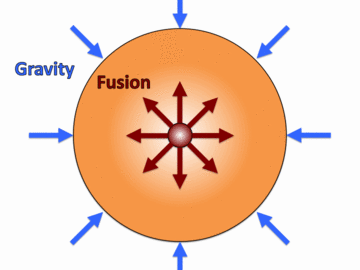
\includegraphics[height=2.5in]{/Users/asnedden/Projects/NCH/Documents/Talks/Nerd_Hour_09_13_2019/images/force_diagram.eps}}
    \put(120, 240){\begin{minipage}[t]{0.7 \linewidth}
    \begin{itemize}
        \item A gravitationaly bound ball of gas that is dense enough for nuclear fusion to occur.
    \end{itemize}
    \end{minipage}}
\end{picture}
\end{frame}


\begin{frame}
\frametitle{What is Nuclear Fusion?}
\pause
\begin{picture}(320,250) 
    \put(0, 78){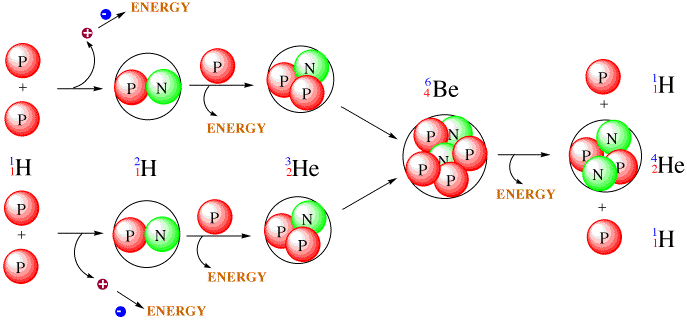
\includegraphics[height=2.25in]{/Users/asnedden/Projects/NCH/Documents/Talks/Nerd_Hour_09_13_2019/images/Hcycle.eps}}
%    \put(120, 240){\begin{minipage}[t]{0.7 \linewidth}
%    \begin{itemize}
%    \end{itemize}
%    \end{minipage}}
\end{picture}
\end{frame}


\begin{frame}
\frametitle{Life Cycle of a Star}
\pause
\begin{picture}(320,250) 
    % https://www.schoolsobservatory.org/learn/astro/stars/cycle
    \put(0, 78){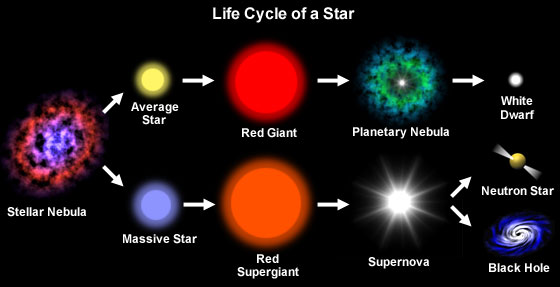
\includegraphics[height=2.25in]{/Users/asnedden/Projects/NCH/Documents/Talks/Nerd_Hour_09_13_2019/images/starcycle.eps}}
    \put(120, 240){\begin{minipage}[t]{0.7 \linewidth}
    \begin{itemize}
        \item Paralax : $\sim$1000 light years % Do finger example. 1200 light years
        \bigskip
        \pause
    \end{itemize}
    \end{minipage}}
    %\put(-10, 108){\includegraphics[height=1.75in]{/Users/asnedden/Projects/NCH/Documents/Talks/Nerd_Hour_2_11_17/figures/Tycho-supernova-xray.eps}}     % Crab Nebula = 
\end{picture}
\end{frame}


\begin{frame}
\frametitle{Life Cycle of a Star}
\pause
\begin{picture}(320,250) 
    %http://astronomy.swin.edu.au/cosmos/H/Hertzsprung-Russell+Diagram
    \put(0, 78){\includegraphics[height=2.25in]{/Users/asnedden/Projects/NCH/Documents/Talks/Nerd_Hour_09_13_2019/images/hrdiagram1.eps}}
    \put(120, 240){\begin{minipage}[t]{0.7 \linewidth}
    \begin{itemize}
        \item Paralax : $\sim$1000 light years % Do finger example. 1200 light years
        \bigskip
        \pause
    \end{itemize}
    \end{minipage}}
    %\put(-10, 108){\includegraphics[height=1.75in]{/Users/asnedden/Projects/NCH/Documents/Talks/Nerd_Hour_2_11_17/figures/Tycho-supernova-xray.eps}}     % Crab Nebula = 
\end{picture}
\end{frame}


% Mention planetary nebulae
\begin{frame}
\frametitle{Stellar Remnants}
White Dwarfs
\pause
\begin{picture}(320,250) 
    %http://astronomy.swin.edu.au/cosmos/H/Hertzsprung-Russell+Diagram
    \put(0, 78){\includegraphics[height=2.25in]{/Users/asnedden/Projects/NCH/Documents/Talks/Nerd_Hour_09_13_2019/images/hrdiagram1.eps}}
    \put(120, 240){\begin{minipage}[t]{0.7 \linewidth}
    \begin{itemize}
        \item Paralax : $\sim$1000 light years % Do finger example. 1200 light years
        \bigskip
        \pause
    \end{itemize}
    \end{minipage}}
    %\put(-10, 108){\includegraphics[height=1.75in]{/Users/asnedden/Projects/NCH/Documents/Talks/Nerd_Hour_2_11_17/figures/Tycho-supernova-xray.eps}}     % Crab Nebula = 
\end{picture}
\end{frame}

% Show image of rotating neutron stars
% Mention Supernova
\begin{frame}
\frametitle{Stellar Remnants}
Neutron Stars :
\pause
\begin{picture}(320,250) 
    %http://astronomy.swin.edu.au/cosmos/H/Hertzsprung-Russell+Diagram
    \put(0, 78){\includegraphics[height=2.25in]{/Users/asnedden/Projects/NCH/Documents/Talks/Nerd_Hour_09_13_2019/images/hrdiagram1.eps}}
    \put(120, 240){\begin{minipage}[t]{0.7 \linewidth}
    \begin{itemize}
        \item Paralax : $\sim$1000 light years % Do finger example. 1200 light years
        \bigskip
        \pause
    \end{itemize}
    \end{minipage}}
    %\put(-10, 108){\includegraphics[height=1.75in]{/Users/asnedden/Projects/NCH/Documents/Talks/Nerd_Hour_2_11_17/figures/Tycho-supernova-xray.eps}}     % Crab Nebula = 
\end{picture}
\end{frame}


% Show image of rotating neutron stars
% Mention Supernova
\begin{frame}
\frametitle{Stellar Remnants}
Black Holes :
\pause
\begin{picture}(320,250) 
    %http://astronomy.swin.edu.au/cosmos/H/Hertzsprung-Russell+Diagram
    \put(0, 78){\includegraphics[height=2.25in]{/Users/asnedden/Projects/NCH/Documents/Talks/Nerd_Hour_09_13_2019/images/hrdiagram1.eps}}
    \put(120, 240){\begin{minipage}[t]{0.7 \linewidth}
    \begin{itemize}
        \item Paralax : $\sim$1000 light years % Do finger example. 1200 light years
        \bigskip
        \pause
    \end{itemize}
    \end{minipage}}
    %\put(-10, 108){\includegraphics[height=1.75in]{/Users/asnedden/Projects/NCH/Documents/Talks/Nerd_Hour_2_11_17/figures/Tycho-supernova-xray.eps}}     % Crab Nebula = 
\end{picture}
\end{frame}



%\end{itemize}
%\end{frame}
\begin{frame}
\printbibliography
\end{frame}

% Backup slides

%\begin{frame}
%\frametitle{Spare slide : Momentum Conservation}
%http://www.preposterousuniverse.com/blog/2010/02/22/energy-is-not-conserved/
%\end{frame}








\end{document}
